% awesome_memory_vla summary deck -- XeLaTeX only (xeCJK). Build: xelatex -interaction=nonstopmode awesome_memory_vla_deck.tex (x2)
\documentclass[aspectratio=169,10pt]{beamer}
\usetheme{Madrid}
\usecolortheme{seahorse}
\setbeamertemplate{navigation symbols}{}
\setbeamertemplate{footline}[frame number]
\usepackage{fontspec}
\usepackage{xeCJK}
\setCJKmainfont{PingFang SC}
\setCJKsansfont{PingFang SC}
\usepackage{amsmath,amssymb,booktabs,mathtools}
\usepackage{graphicx}
\usepackage{hyperref}
\usepackage{tikz}
\usetikzlibrary{arrows.meta,positioning,decorations.pathreplacing}
\usepackage{pgfplots}
\pgfplotsset{compat=1.18}
\definecolor{positive}{HTML}{0173B2}
\definecolor{negative}{HTML}{DE8F05}
\definecolor{emphasis}{HTML}{029E73}
\definecolor{neutral}{gray}{0.55}
\definecolor{cbPurple}{HTML}{CC78BC}
\newcommand{\pos}[1]{\textcolor{positive}{#1}}
\newcommand{\con}[1]{\textcolor{negative}{#1}}
\newcommand{\HL}[1]{\textcolor{emphasis}{\textbf{#1}}}
\setbeamerfont{frametitle}{size=\large,series=\bfseries}

\title[awesome\_memory\_vla]{记忆 VLA：证据消失之后，策略靠什么行动}
\subtitle{Memory for VLA policies: EventVLA · TRACE · SAI, and the 103-paper landscape}
\author{awesome\_memory\_vla · asimfish}
\institute{github.com/asimfish/awesome\_memory\_vla}
\date{2026-09}

\begin{document}

\begin{frame}
\titlepage
\begin{center}
\small 3 篇核心论文深读 · 103 篇文献 · 10 个洞见 · 中英双语报告 · 保版式中文翻译
\end{center}
\end{frame}

% ---------------------------------------------------------------- opening
\begin{frame}{一个数字开场：75.2\% vs 18.0\%}
\begin{columns}[T]
\column{0.50\textwidth}
\textbf{RoboTwin-MeM（8 个双臂任务，必须记住 1--5 个中间关键帧）}
\vspace{4pt}
\begin{center}
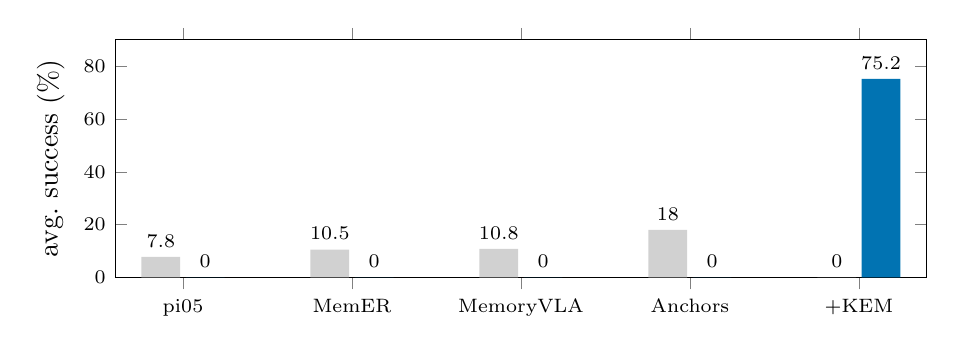
\begin{tikzpicture}
\begin{axis}[ybar, bar width=14pt, width=0.98\textwidth, height=4.6cm,
  symbolic x coords={pi05, MemER, MemoryVLA, Anchors, +KEM}, xtick=data,
  ymin=0, ymax=90, ylabel={avg.\ success (\%)}, nodes near coords,
  every node near coord/.append style={font=\scriptsize}, tick label style={font=\scriptsize}]
\addplot[fill=neutral!40, draw=none] coordinates {(pi05,7.8) (MemER,10.5) (MemoryVLA,10.8) (Anchors,18.0) (+KEM,0)};
\addplot[fill=positive, draw=none] coordinates {(pi05,0) (MemER,0) (MemoryVLA,0) (Anchors,0) (+KEM,75.2)};
\end{axis}
\end{tikzpicture}
\end{center}
{\scriptsize EventVLA, Table 2. Anchors = 初始帧 + 近期帧；+KEM = 再加 5 帧学习选出的事件帧。}
\column{0.46\textwidth}
\textbf{同一个骨干、同一份数据，只多了 5 帧}
\begin{itemize}
\item 标准 VLA 是马尔可夫的：$a_t=\pi(o_t,l)$，默认一切可见
\item 真实任务：掀盖看一眼、读一张数字卡、看别人点一遍顺序 —— \con{证据出现后就消失}
\item 问题不是「要不要记忆」，而是\HL{记什么、何时写、写到哪、存多少}
\end{itemize}
\vspace{4pt}
\textbf{本报告}：三篇 2026 年 6 月的论文从架构 / 模块 / 数据三个层面回答这四问，再放到 103 篇文献里看趋势。
\end{columns}
\end{frame}

\begin{frame}{三篇论文，一个问题，三个层面}
\begin{center}
\begin{tikzpicture}[
  box/.style={draw, rounded corners, minimum width=4.2cm, minimum height=1.55cm, align=center, font=\footnotesize, text width=4.05cm},
  arr/.style={-{Stealth}, thick}]
\node[box, fill=positive!12] (A) {\textbf{EventVLA} (2606.20092)\\架构：KEM 头预测未来关键帧\\存原图，5 帧 FIFO};
\node[box, fill=emphasis!12, right=0.55cm of A] (B) {\textbf{TRACE} (2606.14551)\\模块：外挂 K 槽 latent 记忆\\路径签名寻址};
\node[box, fill=negative!12, right=0.55cm of B] (C) {\textbf{SAI} (2606.16490)\\数据：三阶段非对称课程\\30 步 GRU 历史 token};
\node[draw, rounded corners, fill=white, above=0.7cm of B, minimum width=13.2cm, minimum height=0.9cm, font=\small] (Q)
  {\textbf{决策时刻证据已经不在当前观测里}：被盖住的物体 / 早期分支线索 / 搭档的相位};
\draw[arr] (Q) -- (A); \draw[arr] (Q) -- (B); \draw[arr] (Q) -- (C);
\end{tikzpicture}
\end{center}
\vspace{2pt}
\begin{center}
\small
\begin{tabular}{@{}lccc@{}}
\toprule
 & EventVLA & TRACE & SAI \\
\midrule
看不见的是什么 & 消失的视觉证据 & 早期分支线索 & 搭档内部相位 \\
记忆内容 & 原始图像帧 & 512 维 latent 槽 & GRU 隐状态 \\
何时写 & 学习的关键帧概率 & 每步，门控 & 每步 \\
寻址 & 时间拼接 + 注意力 & 轨迹路径签名 & 无 \\
代价 & 吞吐 2.91$\to$0.94 Hz & +2.1 ms/步 & 干预数据 $\approx$30\% \\
\bottomrule
\end{tabular}
\end{center}
\end{frame}

% ---------------------------------------------------------------- EventVLA
\begin{frame}{EventVLA：把「何时该记住」变成预测问题}
\begin{columns}[T]
\column{0.52\textwidth}
\textbf{记忆} $M_t = A_t \cup E_t$
\begin{itemize}
\item 锚帧 $A_t=\{o_0\}\cup\{o_{t-30},o_{t-15}\}$：全局布局 + 运动线索（规则）
\item 事件帧 $E_t$：KEM 写入，$N_{\max}=5$，FIFO
\item 输入 $I=\mathrm{concat}([A_t,E_{t-1},o_t])$ 直接进 VLM 视觉编码器 —— 「读」就是多帧注意力
\end{itemize}
\textbf{KEM}：与动作头共享最后一层隐状态 $h_t\in\mathbb{R}^{H\times d}$
\[
\hat{\mathbf p}_t=\sigma(\mathrm{MLP}(h_t))\in[0,1]^{H},\quad H=50
\]
写入：$\hat p_t^{\,i}\ge\tau=0.55$ $\Rightarrow$ 存 $o_{t+i}$；1-D NMS（$w=8$）+ 冷却（$C=10$）
\column{0.44\textwidth}
\textbf{训练}
\begin{itemize}
\item 标签：Qwen3-VL-235B 离线看演示输出关键帧步（仿真误差 $<$10 步）
\item 软标签：升余弦核 $y=\tfrac12(1+\cos\pi|t{+}i{-}t^*|/R)$
\item $L=L_{\text{action}}+0.1\,L_{\text{kem}}$
\item 师生课程：真值缓冲 $\to$ 自身预测，$\alpha:1\to0$
\end{itemize}
\vspace{4pt}
\begin{exampleblock}{为什么按整块预测}
事件常在一个动作块中途出现又消失；逐步分类器来不及。共享 $h_t$ 让 KEM 知道策略接下来要做什么，能\HL{预约}一次写入。
\end{exampleblock}
\end{columns}
\end{frame}

\begin{frame}{EventVLA：结果与代价}
\begin{columns}[T]
\column{0.55\textwidth}
\vspace{4pt}
\begin{center}
\small
\begin{tabular}{@{}lrr@{}}
\toprule
方法 & RMBench & RoboTwin-MeM \\
\midrule
$\pi_{0.5}$ & 10.4 & 7.8 \\
MemER / Mem-0 & 8.7 / 42.0 & 10.5 / 0.0 \\
MemoryVLA (QwenOFT) & 41.7 & 10.8 \\
EventVLA 仅锚帧 & \textbf{67.8} & 18.0 \\
EventVLA 锚帧 + KEM & -- & \textbf{75.2} \\
\midrule
\multicolumn{3}{@{}l}{\textit{消融（RoboTwin-MeM）}} \\
隐式记忆库（latent） & & \con{24.9} \\
硬标签 / 去 NMS & & 48.8 / 53.4 \\
$N_{\max}=2$ & & 32.0 \\
动作块 30 / 15 & & 31.1 / \con{13.6} \\
\bottomrule
\end{tabular}
\end{center}
{\scriptsize 真机 ARX ACONE 4 任务 $\times$ 20：\HL{90 / 60 / 90 / 75}，$\pi_{\text{MEM}}$ 50 / -- / 30 / 40。}
\column{0.42\textwidth}
\textbf{三个值得记住的数字}
\begin{itemize}
\item \HL{24.9 vs 75.2}：同框架只换记忆表征，原图胜 latent —— 至少在要同时记 3--5 个视觉细节时
\item \con{13.6}：动作块从 50 缩到 15，KEM 的前瞻随之崩塌 —— 记忆机制与块长度耦合
\item \con{0.94 Hz}：多帧输入把吞吐压到基座的 1/3
\end{itemize}
\vspace{4pt}
\textbf{留意}：KEM 未在 RMBench 上测；两套基准同出 RoboTwin 系；5 帧 FIFO 对 $>$10 分钟任务会饱和。
\end{columns}
\end{frame}

% ---------------------------------------------------------------- TRACE
\begin{frame}{TRACE：用「走过的路」给记忆编地址}
\begin{columns}[T]
\column{0.52\textwidth}
\textbf{延迟证据}：短窗口下 $x_{t-w+1:t}\approx x'_{t-w+1:t}$ 但 $a^*_t(\mathcal H_t)\ne a^*_t(\mathcal H'_t)$
\vspace{4pt}
\textbf{内容与地址分离}
\begin{itemize}
\item 内容 $e_t=\phi_x(x_t)$：多视角视觉 + 本体
\item 地址：17 维状态路径的深度-3 路径签名，$17+17^2+17^3=5219$ 维，加增量 $\delta_t=\xi_t-\xi_{t-1}$
\item 性质：对时间重参数化、常数偏移\pos{不变}，对\HL{顺序}敏感；流式 0.52 ms
\end{itemize}
\textbf{槽记忆} $M_t\in\mathbb{R}^{K\times 512}$，$K=4/6$
\begin{align*}
\omega_{t,k}&=\mathrm{softmax}_k\!\big(\tfrac{(W_Q\rho_t)^\top W_K\bar m_{t-1,k}}{\tau\sqrt{d_r}}\big)\\
m_{t,k}&=(1-\beta_{t,k})\,m_{t-1,k}+\beta_{t,k}\,\tilde m_{t,k}
\end{align*}
\column{0.44\textwidth}
\textbf{适配器只做翻译}
\begin{itemize}
\item ACT：槽 $\to$ 512 维记忆 token 拼进注意力 memory（+0.79 M）
\item Diffusion：池化 $\to$ 零初始化 MLP $\to$ 加性全局条件（+16.03 M）
\item 共享更新器 11.91 M；骨干、动作头、损失都不改
\end{itemize}
\vspace{4pt}
\textbf{三个稳定器}（只作用于记忆）
\begin{itemize}
\item $L_{\text{bal}}$ 防槽塌缩 · $L_{\text{ent}}$ 防弥散写入 · $L_{\text{cons}}$ 防读写失配
\item 去掉它们：69.23 $\to$ 66.10
\end{itemize}
\end{columns}
\end{frame}

\begin{frame}{TRACE：结果与诊断}
\begin{columns}[T]
\column{0.50\textwidth}
\vspace{4pt}
\begin{center}
\small
\begin{tabular}{@{}lr@{}}
\toprule
方法（5 真机任务，阶段进度 \%） & 平均 \\
\midrule
ACT / Diffusion Policy & 25.50 / 25.00 \\
$\pi_{0.5}$（同数据微调） & 50.47 \\
GRU 循环记忆 & 45.83 \\
Transformer 历史上下文 & 52.10 \\
LRU 外部记忆 & 53.93 \\
检索提示记忆（MAP-VLA 式） & 56.30 \\
\textbf{TRACE（回归 / 扩散）} & \textbf{69.23} / 59.53 \\
\midrule
只有签名（不存视觉证据） & 45.50 \\
无路由槽 / 去增量 & 52.17 / 61.43 \\
\bottomrule
\end{tabular}
\end{center}
\column{0.46\textwidth}
\textbf{历史变换诊断}（归一化到完整 TRACE）
\begin{center}
\small
\begin{tabular}{@{}lrr@{}}
\toprule
变换 & 路由相似 & 分支一致 \\
\midrule
时间重采样 & 92.4 & 96.0 \\
速度抖动 & 89.8 & 94.7 \\
状态偏移 & 91.2 & 95.1 \\
稀疏采样 & 86.5 & 92.3 \\
\con{顺序反转} & \con{37.8} & \con{41.6} \\
\bottomrule
\end{tabular}
\end{center}
\begin{alertblock}{可推广的方法论}
同样的分岔点画面、同样的权重，把历史倒放，记忆读出就变了 —— 「记忆在用有序历史」从假设变成测量。
\end{alertblock}
\end{columns}
\end{frame}

% ---------------------------------------------------------------- SAI
\begin{frame}{SAI：搭档看不全，历史和课程都要替它补}
\begin{columns}[T]
\column{0.50\textwidth}
\textbf{设定}：两台双臂移动操作机器人，无通信，各自局部观测 $a_i^t\sim\pi_i(\cdot|o_i^t)$；单遥操作者
\vspace{4pt}
\begin{center}
\begin{tikzpicture}[
  st/.style={draw, rounded corners, minimum width=2.15cm, minimum height=1.15cm, align=center, font=\scriptsize, text width=2.05cm},
  arr/.style={-{Stealth}, thick}]
\node[st, fill=positive!12] (s1) {\textbf{阶段 1}\\A 与顺从人类搭档\\搭档区域随机化};
\node[st, fill=emphasis!12, right=0.45cm of s1] (s2) {\textbf{阶段 2}\\冻结 A，人遥操 B\\A 加有界扰动};
\node[st, fill=negative!12, right=0.45cm of s2] (s3) {\textbf{阶段 3}\\A+B 联合部署\\对 A 稀疏 DAgger 干预};
\draw[arr] (s1) -- (s2); \draw[arr] (s2) -- (s3);
\end{tikzpicture}
\end{center}
$\pi_A^{(3)}=\mathrm{BC}(\mathcal D_A^{\text{solo}}\cup\mathcal D_A^{\text{int}})$，干预 $\approx$ 基线数据 30\%，动作维掩码

\vspace{2pt}
\textbf{策略}：ACT + 冻结 DINOv3，30 步历史（12 帧对数采样 $\to$ GRU），级联底盘 $\to$ 手臂头
\column{0.46\textwidth}
\begin{center}
\small
\begin{tabular}{@{}llrrr@{}}
\toprule
任务 & 方法 & 成功 & 相位同步 & 让步 \\
\midrule
Bed-throw & 独立 & 23.3 & 30.8 & 26.7 \\
 & \textbf{SAI} & \textbf{53.3} & \textbf{62.5} & \textbf{68.3} \\
Tablecloth & 独立 & 43.3 & 54.4 & 46.7 \\
 & \textbf{SAI} & \textbf{66.7} & \textbf{68.9} & \textbf{70.0} \\
Laundry & 独立 & 50.0 & 51.7 & 31.7 \\
 & \textbf{SAI} & \textbf{70.0} & \textbf{73.3} & \textbf{71.7} \\
Painting & 独立 & 33.3 & 42.7 & 34.4 \\
 & \textbf{SAI} & \textbf{56.7} & \textbf{74.7} & \textbf{68.9} \\
\bottomrule
\end{tabular}
\end{center}
\begin{itemize}
\item 阶段 2 抬相位同步，阶段 3 抬让步；成功率是两者之和
\item \HL{历史 token}：提前松手 64.5\% $\to$ 16.1\% —— 单帧分不清「搬运中」与「该松手」
\item 换 Diffusion 头同样有效（23.5 $\to$ 52.9）
\end{itemize}
\end{columns}
\end{frame}

% ---------------------------------------------------------------- landscape
\begin{frame}{放到 103 篇里看：2026 年 6--8 月的爆发}
\begin{center}

\includegraphics[width=0.96\textwidth]{../assets/timeline.svg.pdf}
\end{center}
\vspace{-4pt}
{\small 2025 全年 24 篇；2026 年 1--5 月 23 篇；\HL{6 月 20 篇、7 月 10 篇、8 月 17 篇}。春天落地的 RMBench / RoboMME / RoboMemArena 给了方法论文共同的靶子。}
\end{frame}

\begin{frame}{五个技术家族 + 六个必答问题}
\begin{columns}[T]
\column{0.42\textwidth}
\textbf{家族}（README 第 3--7 节）
\begin{enumerate}
\item 事件 / 关键帧记忆：EventVLA, KEMO, UniMem, WeaveLA
\item 稠密压缩历史：MemoryVLA, NativeMEM, StreamPI, TempoFit
\item latent / 循环 / 槽：TRACE, $\mu$VLA, Chronos, TFP, GMP
\item 双系统 / 智能体 / 符号：MEM, MemER, AGM, HyMeS, BATON
\item 世界模型内的记忆：MemoryWAM, MemoryVAM
\end{enumerate}
\vspace{2pt}
第六个方向：\con{多机器人搭档记忆}（SAI, HATS, Duet），几乎空白。
\column{0.55\textwidth}
\begin{center}
\small
\begin{tabular}{@{}lll@{}}
\toprule
问题 & EventVLA & TRACE \\
\midrule
存什么 & 原图 & 512-D latent \\
何时写 & \HL{学习触发} + NMS & 每步，门控 \\
寻址 & 时间拼接 & \HL{轨迹签名} \\
存多少 & 5 + 锚帧 & K = 4/6 \\
接在哪 & 视觉编码器输入 & 动作头前适配器 \\
监督 & 235B 标注 + 软标签 & 三项稳定器 \\
\bottomrule
\end{tabular}
\end{center}
\vspace{2pt}
{\small 两个极端在同一个月被占住：EventVLA 押「何时写」，TRACE 押「从哪读」。\HL{既学写入时机、又学寻址}的中间地带还是空的。}
\end{columns}
\end{frame}

\begin{frame}{跨基准证据：没有一种记忆在所有基准上领先}
\begin{center}
\small
\begin{tabular}{@{}llr@{}}
\toprule
基准 & 方法 & 数字 \\
\midrule
RMBench (9 任务) & $\pi_{0.5}$ / Mem-0 / MemoryVLA & 10.4 / 42.0 / 41.7 \\
 & ChainVLA / EventVLA 仅锚帧 / \textbf{Chronos} & 62.8 / 67.8 / \textbf{73.6} \\
RoboMME (16 任务) & $\pi_{0.5}$ / FrameSamp+Modul / \textbf{PonderPounce 9B} & 17.93 / 44.51 / \textbf{60.83} \\
RoboMemArena (26 任务) & $\pi_{0.5}$ / \textbf{HyMeS}（累计 / 任务） & 52.5 / 41.3 $\to$ \textbf{66.2 / 60.1} \\
MIKASA-Robo (32 任务) & MemoryVLA / $\mu$VLA（5 训练任务） & 41.2 / 0.42 $\to$ 0.84 \\
真机瞬态证据 & EventVLA / KEMO / UniMem & 90--60 / +23.6 / 80.0 vs 43.5 \\
真机延迟证据 & TRACE (ACT) vs $\pi_{0.5}$ & 69.23 vs 50.47 \\
\bottomrule
\end{tabular}
\end{center}
\vspace{2pt}
\begin{itemize}
\item RMBench 上「初始帧 + 近期帧」已到 67.8 $\Rightarrow$ 记忆需求偏浅；Chronos 73.6 靠全历史 SSM 而非事件记忆
\item RoboMME / RoboMemArena 榜首是\HL{双系统}（PonderPounce, HyMeS, BATON）：计数与过程记忆目前符号状态更稳
\item 真机瞬态视觉证据上\HL{端到端事件记忆}绝对成功率最高
\item 各基准口径不同，跨论文数字\con{不可直接比较}
\end{itemize}
\end{frame}

% ---------------------------------------------------------------- insights
\begin{frame}{十个洞见（1--5）}
\begin{enumerate}
\item \textbf{前沿从「存多少」转到「何时写」}：EventVLA / KEMO / UniMem / WeaveLA / MemoryWAM / TFP 从不同架构同时转向事件驱动稀疏写入；TFP 事件附近写入增益 $\approx$6$\times$
\item \textbf{机理}（Present but Not Remembered）：冻结 VLA 里的历史是当前帧的\con{冗余副本}，只属于过去的信息几乎不存在 $\Rightarrow$ 记忆增强应注入\HL{过去独有}的信息
\item \textbf{原图 vs latent 取决于要恢复多少比特}：EventVLA 24.9 vs 75.2（3--5 个视觉细节）与 TRACE 69.23（1--2 比特分支变量）并不矛盾
\item \textbf{寻址被低估}：TRACE 让写入时刻与读取时刻有稳定对应（保序 $\sim$90，倒序 37.8）；分支若不对应运动差异则退化
\item \textbf{长上下文没那么脆，但虚假相关是真的}：Agarwal et al.\ vs PTP / GMP（+30.1）/ HALO —— 能否用长窗口取决于监督是否把注意力引向任务相关历史
\end{enumerate}
\end{frame}

\begin{frame}{十个洞见（6--10）}
\begin{enumerate}
\setcounter{enumi}{5}
\item \textbf{可靠性来自有纪律的状态更新，不是容量}：AGM 验证后推进、EventVLA NMS + 冷却、TRACE 门控写入、BATON 验证器 —— \HL{记忆写入应是带验证的事务}
\item \textbf{双系统在计数与过程记忆上仍领先}：PonderPounce（p50 78 ms 刷新 / 25 ms 动作）在缩小延迟劣势；分界线变成「哪类信息放哪一层」
\item \textbf{记忆成本趋近于零}：NativeMEM 每帧 1 token、TempoFit 免训练、StreamPI 零参数、DySta 2$\times$ 加速；EventVLA 的 3$\times$ 延迟会被后继者先优化
\item \textbf{多机器人是同一问题的另一张脸}：搭档相位 = 从历史推断的隐变量；SAI 只有 30 步 GRU，\con{无人}把显式记忆用于搭档状态估计
\item \textbf{评测在分裂，诊断在成熟}：一年 12 套基准；TRACE 顺序反转负对照、探针 + 因果干预、TFP 隐状态干预 $\Rightarrow$ 同时报告「成功率」与「记忆用了什么」
\end{enumerate}
\end{frame}

\begin{frame}{开放问题与我们的下一步}
\begin{columns}[T]
\column{0.48\textwidth}
\textbf{开放问题}
\begin{itemize}
\item 缓冲区饱和：5 帧 FIFO（$>$10 min）；固定槽 2$\times$ 历史一致性 0.928
\item 签名维度立方增长：深度 4 $\to$ 88{,}740 维；高维人形需 log-signature
\item 写入触发的监督：235B 标注 / 规则 / 分类器 / rollout 结果，无跨任务对照
\item 记忆与动作块长度耦合（75.2 $\to$ 13.6）
\item 错误记忆的安全性（AGM）
\item 基准统一：RoboMME 四类 + RoboTwin-MeM 的 $n$ + TRACE 阶段进度
\end{itemize}
\column{0.48\textwidth}
\textbf{研究方向}
\begin{enumerate}
\item \HL{前瞻写入 $\times$ 轨迹寻址}：KEM 决定何时写，签名决定写到哪；在 RoboTwin-MeM 与 TRACE 任务上同时验证
\item \HL{搭档相位记忆}：SAI 的 30 步 GRU $\to$ 签名槽记忆（键 = A 的轨迹，内容 = 对 B 的观测）
\item \HL{记忆诊断基准}：RoboMME 四类任务各配保序 / 破序变换，路由相似度成为标准报告项
\item \HL{写入触发的跨任务迁移}：同骨干对照学习 / 规则 / 分类器三种触发
\end{enumerate}
\end{columns}
\end{frame}

\begin{frame}{三句话带走}
\begin{enumerate}
\item \textbf{记忆的四问}（记什么 / 何时写 / 写到哪 / 存多少）比「要不要记忆」重要；EventVLA 与 TRACE 各答了一问的极端，中间地带空着。
\item \textbf{表征跟信息量走}：要恢复多个视觉细节用原图（75.2 vs 24.9），要恢复分支变量用槽（69.23），要计数用符号（AGM / HyMeS）。
\item \textbf{用诊断代替猜测}：把历史倒放看记忆读出变不变（TRACE），用探针看历史是否只是当前帧的副本（Liao \& Cao）。
\end{enumerate}
\vspace{6pt}
\begin{center}
\small 仓库：\texttt{github.com/asimfish/awesome\_memory\_vla} · 深读报告 \texttt{reports/} · 论文笔记 \texttt{notes/} · 翻译 \texttt{papers/zh/}
\end{center}
\end{frame}

\begin{frame}{References}
\small
\begin{thebibliography}{9}
\bibitem{eventvla} Yang et al. EventVLA: Event-Driven Visual Evidence Memory for Long-Horizon VLA Policies. arXiv:2606.20092, 2026.
\bibitem{trace} Li, Qiu, Chen, Ren, Zhi. TRACE: Trajectory-Routed Causal Memory for Delayed-Evidence Visuomotor Imitation. arXiv:2606.14551, 2026.
\bibitem{sai} Chen, Qiu, Li, Zhou, Ren, Zhi. Robots that Collaborate: Sequential Asymmetric Imitation for Learning Coupled Robot Policies. arXiv:2606.16490, 2026.
\bibitem{pnr} Liao, Cao. Present but Not Remembered: Auditing How Frozen VLAs Encode, Deploy, and Steer Visual History. arXiv:2607.03372, 2026.
\bibitem{robomme} Dai et al. RoboMME: Benchmarking and Understanding Memory for Robotic Generalist Policies. arXiv:2603.04639, 2026.
\bibitem{agm} Gao et al. AGM: Achievement-Grounded Memory for Closed-Loop Agents with Frozen VLA Policies. arXiv:2608.29537, 2026.
\bibitem{chronos} Zhou et al. Chronos: A Physics-Informed Full-History Framework for Non-Markovian Long-Horizon Manipulation. arXiv:2606.30318, 2026.
\end{thebibliography}
\end{frame}

\begin{frame}
\begin{center}
{\Large 谢谢 · Thank you}\\[8pt]
\small 所有数字只取自原文；不同论文的数字建立在各自任务集与口径上，不可直接比大小。
\end{center}
\end{frame}

\appendix
\begin{frame}{Backup Slides}\end{frame}

\begin{frame}{Backup: EventVLA 超参与 RoboTwin-MeM 任务}
\begin{columns}[T]
\column{0.46\textwidth}
\scriptsize
\begin{tabular}{@{}ll@{}}
\toprule
设置 & 仿真 / 真机 \\
\midrule
基座 & Qwen3-VL-4B (QwenOFT) / $\pi_{0.5}$ \\
动作块 $H$ & 50 / 50 \\
锚帧（仿真） & $o_0,\,o_{t-30},\,o_{t-15}$ \\
锚帧（真机） & $o_0,\,o_{t-60},\,o_{t-40},\,o_{t-20}$ \\
$\tau$, $N_{\max}$, $w$, $C$, $\lambda$ & 0.55, 5, 8, 10, 0.1 \\
训练步数 & 80k / 60k \\
\bottomrule
\end{tabular}
\column{0.50\textwidth}
\small
\begin{tabular}{@{}lrr@{}}
\toprule
任务 & $n$ & 平均步数 \\
\midrule
Press Button Keyframe & 2--5 & 430 \\
Pick the Unhidden Block & 3 & 699 \\
Rearrange Blocks Hard & 1 & 879 \\
Pick Objects in Order & 3 & 1124 \\
Find Seal and Seal Stamp & 1--4 & 1338 \\
Reproduce Route & 4 & 1417 \\
Put Back Block Hard & 2 & 1468 \\
Cover Blocks Hard & 4 & 1544 \\
\bottomrule
\end{tabular}
\end{columns}
\end{frame}

\begin{frame}{Backup: TRACE 任务、参数与延迟}
\begin{columns}[T]
\column{0.46\textwidth}
\scriptsize
\begin{tabular}{@{}lrrr@{}}
\toprule
任务 & 演示 & 回合长度 & 子任务/阶段 \\
\midrule
Tool & 100 & 2910 帧 (97 s) & 2/4 \\
Book & 150 & 1392 帧 (46 s) & 3/4 \\
Laundry & 60 & 2220 帧 (74 s) & 2/4 \\
Cable & 30 & 1770 帧 (59 s) & 1/4 \\
Medicine & 60 & 1759 帧 (59 s) & 2/4 \\
\bottomrule
\end{tabular}
\column{0.50\textwidth}
\scriptsize
\begin{tabular}{@{}lrr@{}}
\toprule
 & 回归 & 扩散 \\
\midrule
基座前向 (ms) & 5.90 & 118.00 \\
签名 / 槽更新 / 读出 & 0.52 / 0.90 / 0.58 & 同 \\
TRACE 总开销 (ms) & 2.11 & 2.15 \\
占比 & 35.8\% & 1.8\% \\
新增参数 & 12.69 M (+24.6\%) & 27.94 M (+10.3\%) \\
\bottomrule
\end{tabular}
\vspace{4pt}
{\scriptsize RTX 5090, PyTorch 2.9.1。签名深度 $p=3$，$d_{\text{sig}}=5219$；$p=4$ 为 88{,}740。}
\end{columns}
\end{frame}

\begin{frame}{Backup: SAI 架构消融与骨干无关性}
\begin{columns}[T]
\column{0.44\textwidth}
\scriptsize
\begin{tabular}{@{}llr@{}}
\toprule
失败模式 & 变体 & 失败率 \\
\midrule
提前松手 (Laundry) & 无历史 / 有历史 & 64.5 / \textbf{16.1} \\
提前下放 (过渡) & 无级联 / 有级联 & 51.6 / \textbf{9.7} \\
\bottomrule
\end{tabular}
\column{0.52\textwidth}
\scriptsize
\begin{tabular}{@{}llrrr@{}}
\toprule
动作头 & 流程 & 成功 & 同步 & 让步 \\
\midrule
ACT & 独立 / SAI & 33.3 / 56.7 & 42.7 / 74.7 & 34.4 / 68.9 \\
Diffusion & 独立 / SAI & 23.5 / 52.9 & 35.2 / 62.2 & 30.7 / 76.9 \\
\bottomrule
\end{tabular}
\end{columns}
\vspace{6pt}
{\small Painting Transport；ACT 30 次 / Diffusion 34 次 rollout。历史与级联头提升局部执行可靠性，协作收益来自数据课程（三个流程共用同一架构）。}
\end{frame}

\end{document}
